\documentclass[conference]{IEEEtran}
\IEEEoverridecommandlockouts
% The preceding line is only needed to identify funding in the first footnote. If that is unneeded, please comment it out.
\usepackage{cite}
\usepackage{amsmath,amssymb,amsfonts}
\usepackage{algorithmic}
\usepackage{graphicx}
\usepackage{textcomp}
\usepackage{booktabs}
\usepackage{threeparttable}
\usepackage{siunitx}
\usepackage{multirow}

\usepackage{xcolor}
\def\BibTeX{{\rm B\kern-.05em{\sc i\kern-.025em b}\kern-.08em
    T\kern-.1667em\lower.7ex\hbox{E}\kern-.125emX}}


\begin{document}

\title{MACCA: Controle Adaptativo de Taxa de Bits para Jogos em Nuvem no Sunshine}

\author{\IEEEauthorblockN{César de Paula Morais}
\IEEEauthorblockA{\textit{Departamento de Ciência da Computação} \\
\textit{Universidade Federal de Minas Gerais}\\
Belo Horizonte, Brasil \\
cesarmorais@dcc.ufmg.br}
\and
\IEEEauthorblockN{Dr. Luiz Filipe Menezes Vieira}
\IEEEauthorblockA{\textit{Departamento de Ciência da Computação} \\
\textit{Universidade Federal de Minas Gerais}\\
Belo Horizonte, Brasil \\
lfvieira@dcc.ufmg.br}
}

\maketitle


\begin{abstract}
Jogos em nuvem impõem requisitos rigorosos de latência e de
perda de pacotes que a rede doméstica raramente respeita de
forma consistente, comprometendo a experiência do usuário
sob variações súbitas de capacidade. Este artigo investiga a
aplicação de um controlador adaptativo de taxa de bits ao
servidor open-source \emph{Sunshine}, denominado MACCA, baseado em um esquema
\emph{Additive Increase, Multiplicative Decrease} (AIMD)
estendido com duas primitivas do algoritmo CUBIC: a curva
cúbica de recuperação após reduções de taxa e o mecanismo de
\emph{fast convergence}. O controlador proposto opera
exclusivamente a partir do RTT mantido pela biblioteca ENet
no canal de controle, sem qualquer modificação no protocolo
Moonlight ou cooperação adicional do cliente. Foi avaliado
em uma campanha experimental envolvendo seis cenários de
degradação de rede emulada e dois controladores de
referência. Os resultados mostraram que a abordagem proposta
reduz o pico de RTT em cinco dos seis cenários, com a maior
queda atingindo 43\%, e o tempo total acumulado em
\emph{stall} em cinco dos seis cenários, com queda de até
61\%, ao custo de uma elevação sistemática do RTT mediano.
Esses achados caracterizam um trade-off entre desempenho na
cauda da distribuição de latência e desempenho no regime
estacionário, e indicam que algoritmos de controle de
congestionamento projetados para amostragem densa exigem
ajuste estrutural, e não apenas reparametrização, ao serem
transpostos para regimes de cadência reduzida.
\end{abstract}

\begin{IEEEkeywords}
jogos em nuvem, controle de congestionamento, taxa de bits adaptativa,
AIMD, CUBIC, MACCA, Sunshine, streaming de jogos.
\end{IEEEkeywords}

\section{Introdução}\label{sec:introducao}

Em cloud gaming, o servidor executa o jogo e transmite ao cliente apenas o vídeo codificado, permitindo o acesso a títulos de alto custo computacional em dispositivos modestos.
Essa separação transfere para a rede o ônus de sustentar uma
experiência tradicionalmente local ao usuário, impondo
requisitos rigorosos: latência de ida e volta inferior a
\SI{100}{\milli\second} para jogos de ação e taxa de perda
abaixo de 1\%~\cite{baldovino2022}. A rede doméstica raramente
respeita esses limiares de forma consistente, e qualquer
variação súbita de capacidade manifesta-se imediatamente como
travamento visual ou perda de sincronia. As plataformas
comerciais dominantes contornam parcialmente o problema com
investimento maciço em infraestrutura, ao custo de um modelo
operacional baseado em assinatura, catálogo restrito ao
licenciamento da operadora, hardware proprietário e ausência
de controle do usuário sobre a sessão.

O \emph{Sunshine}~\cite{sunshine} é um servidor open-source de \emph{streaming}
de jogos compatível com o protocolo NVIDIA GameStream e
cliente Moonlight~\cite{moonlight}, mantido sob a licença GPL-3.0, e
constitui-se como a alternativa \emph{self-hosted} mais
adotada. Atualmente, opera com taxa de bits negociada uma
única vez ao início da sessão, sem qualquer mecanismo de
reação a degradação observada do canal. Diante de constrições
de banda, o comportamento resultante combina estouro de
\emph{buffer} no gargalo, inflação contínua do RTT e cascatas
sucessivas de quadros IDR. Os trabalhos correlatos mais
próximos~\cite{alos2019,abragame,gcc} resolvem o problema do
controle adaptativo de taxa de bits em contextos próprios,
mas todos pressupõem extensão do protocolo de \emph{streaming},
cooperação ativa do cliente ou sincronização de relógio,
requisitos incompatíveis com o protocolo Moonlight e sua base
instalada.

Neste artigo, propomos e avaliamos o MACCA (\emph{Multi-state
AIMD with Cubic Convergence Adaptation}), um
controlador adaptativo de taxa de bits para o servidor
Sunshine, baseado exclusivamente em sinais já disponíveis no
servidor e sem qualquer modificação no cliente. O controlador
estende um esquema AIMD clássico com duas primitivas do
algoritmo CUBIC~\cite{cubic}: a curva cúbica de recuperação
após reduções de taxa e o mecanismo de \emph{fast convergence}
para atualização do teto de referência. As contribuições são
três. \emph{Primeiro}, o projeto e a implementação do
controlador, integrado à árvore de código do Sunshine.
\emph{Segundo}, uma campanha experimental sobre seis cenários
de degradação de rede e três controladores, em que o AIMD
CUBIC reduz o pico de RTT em cinco dos seis cenários, com a
maior queda alcançando 43\%, e o tempo total acumulado em
\emph{stall} em cinco dos seis cenários, com queda de até
61\%, ao custo de uma elevação sistemática do RTT mediano e
sem dominar a referência adaptativa em todas as dimensões.
Esse resultado caracteriza um trade-off entre cauda e regime
estacionário da distribuição de latência que se mostra
fundamental para o posicionamento de controladores
adaptativos em jogos em nuvem. \emph{Terceiro}, um achado
estrutural sobre a adaptação do CUBIC a regimes de cadência
reduzida: a forma literal da curva, projetada para amostragem
por~ACK, mostra-se empiricamente inferior à variante
simplificada aqui adotada quando aplicada a 1~Hz, indicando
que algoritmos de controle de congestionamento entre regimes
de cadência distintos exigem ajuste estrutural, e não apenas
reparametrização.

A diferenciação em relação ao estado da arte concentra-se na
ausência de requisitos sobre o cliente e o protocolo,
discutida em detalhe no Capítulo~\ref{sec:referencial}.

O Capítulo~\ref{sec:referencial} apresenta o referencial
teórico e o posicionamento contra os trabalhos correlatos. O
Capítulo~\ref{sec:contribuicao} descreve o controlador
proposto. O Capítulo~\ref{sec:metodologia} detalha o
\emph{testbed} físico, os cenários de degradação e o
protocolo experimental. O Capítulo~\ref{sec:resultados}
apresenta os resultados, incluindo a análise de sensibilidade
ao design da curva. O Capítulo~\ref{sec:conclusao} retoma os
achados centrais e discute trabalhos futuros.


\section{Referencial Teórico}\label{sec:referencial}

Esta seção apresenta uma revisão sistemática da literatura
relevante para controle adaptativo de taxa de bits em jogos em
nuvem. A revisão foi estruturada em seis eixos temáticos
complementares, conduzidos do mais geral ao mais específico:
caracterização do problema de rede em jogos em nuvem, codecs de
vídeo e reconfiguração em tempo de execução, controle de
congestionamento na herança do TCP, controle adaptativo para
mídia em tempo real, o trabalho mais próximo da contribuição
proposta, e o servidor \emph{Sunshine} como plataforma de
contribuição.

\subsection{Jogos em Nuvem como Problema de Rede}

Jogos em nuvem (\emph{cloud gaming}) consistem em executar o
jogo em um servidor remoto, capturar a saída de vídeo do jogo,
codificá-la em tempo real e transmiti-la a um cliente leve, que
decodifica e exibe os quadros enquanto envia comandos de entrada
de volta ao servidor. A arquitetura delega ao
servidor a carga computacional (GPU, codec), reduzindo o cliente
a um decodificador de vídeo — viabilizando jogos de alto custo
em hardware modesto.

Esta separação, no entanto, impõe requisitos rigorosos ao canal de rede. A revisão sistemática conduzida por Baldovino~\cite{baldovino2022}, abrangendo 33 estudos publicados entre 2017 e 2022, consolida os limiares tradicionalmente adotados pela literatura para caracterizar as condições necessárias à operação adequada de sistemas de cloud gaming: latência de ida e volta inferior
a \SI{100}{\milli\second} para jogos de ação, taxa de perda
inferior a 1\%, e tempo de resposta total (\emph{response time})
entre 100 e \SI{150}{\milli\second}. Acima desses limiares, a
experiência do usuário degrada de forma perceptível e, em casos
extremos, torna o jogo injogável.

A importância desses limiares está associada a uma característica fundamental do próprio meio. Diferentemente do \emph{streaming} de vídeo sob demanda, em que \emph{buffers} de alguns segundos conseguem mascarar variações da rede de forma praticamente transparente ao usuário, aplicações de cloud gaming operam com \emph{buffers} reduzidos, geralmente limitados a um ou dois quadros, para manter a interatividade. Como consequência, atrasos, perdas de pacotes ou variações na latência (\emph{jitter}) são rapidamente refletidos na qualidade percebida, manifestando-se na forma de travamentos, \emph{tearing} ou perda de sincronização.

Hong et al.~\cite{hong2015} avaliaram três jogos executados a 720p sobre o \emph{GamingAnywhere} e observaram que o MOS (\emph{Mean Opinion Score}) tende a saturar em torno de \SI{2}{\mega\bit\per\second}. Acima desse valor, aumentos na taxa de bits produzem ganhos perceptuais limitados; abaixo dele, a qualidade percebida se deteriora rapidamente. Esse comportamento reforça a importância de considerar métricas de cauda, como valores de pico e percentis elevados (p99), em vez de medidas centrais como a mediana, abordagem que será retomada no Capítulo~\ref{sec:metodologia}.

Como o processo de codificação é executado no servidor, este possui controle direto sobre a principal variável reconfigurável do pipeline: a taxa de bits-alvo do codificador. O servidor constitui, portanto, o ponto mais natural para a implementação da política de adaptação, dispensando mecanismos adicionais de cooperação por parte do cliente ou da infraestrutura de rede. Essa observação motiva o recorte adotado neste trabalho, detalhado no Capítulo~\ref{sec:contribuicao}.


% TODO - avaliar se vale colocar mais referencias nessa parte
\subsection{Codecs de Vídeo e Reconfiguração em Tempo de Execução}

A compressão de vídeo em jogos em nuvem é dominada pelos padrões
H.264, HEVC (H.265) e, mais recentemente, AV1, todos baseados em
predição temporal entre quadros. Três tipos de quadros compõem
um fluxo típico: quadros-I (\emph{intra-coded}), codificados de
forma independente; quadros-P (\emph{predicted}), que dependem
de quadros anteriores; e quadros-B (\emph{bidirectional}),
ausentes em jogos em nuvem por exigirem buffer adiante. Dentro
da categoria de quadros-I, os quadros IDR (\emph{Instantaneous
Decoder Refresh}) zeram a referência do decodificador, isolando
o erro de propagação após perdas — funcionando como mecanismo de
recuperação de último recurso quando outras escadas de proteção
(FEC, retransmissão seletiva) falham.

Entretanto, o custo dos quadros IDR é alto: por carregarem todo o
conteúdo do quadro de forma independente, IDRs são
substancialmente maiores que quadros-P, gerando picos abruptos
no tráfego de saída. Quando o canal já se encontra próximo da
saturação, a inserção de um IDR pode provocar enfileiramento no
gargalo, elevando o RTT (\emph{round-trip time}) e desencadeando
uma cascata: o cliente, ao não receber o IDR a tempo, solicita
outro, perpetuando o ciclo. Reduzir a frequência de IDRs é,
portanto, um objetivo indireto, mas relevante, do controle
adaptativo de taxa de bits.

A reconfiguração dinâmica da taxa de bits do codificador é
suportada pelos principais \emph{encoders} de hardware modernos. O trabalho de Hong et al.~\cite{hong2015}
foi pioneiro em estender o servidor open-source
\emph{GamingAnywhere} (GA) — antecessor direto do Sunshine — com
suporte a reconfiguração de codec em tempo de execução, antes
indisponível na plataforma. O presente trabalho herda
diretamente esta linha: opera sobre uma plataforma open-source
sucessora do GA e contribui exatamente com a política de decisão
que aciona essa reconfiguração — não com a reconfiguração em si,
que o Sunshine já suporta.

\subsection{Controle de Congestionamento: do TCP ao Streaming}

O controle de congestionamento na Internet é historicamente baseado no TCP. A família clássica de algoritmos TCP --- incluindo Reno, NewReno e SACK --- segue a política AIMD (\emph{Additive Increase, Multiplicative Decrease}), em que a janela de congestionamento cresce de forma aditiva na ausência de perdas e é reduzida multiplicativamente quando uma perda é detectada. Embora estável e amplamente estudada, essa estratégia apresenta limitações em redes com alto produto banda-atraso. Em um enlace de \SI{10}{\giga\bit\per\second} e RTT de \SI{100}{\milli\second}, por exemplo, o TCP clássico levaria aproximadamente 1,4 horas para recuperar a taxa de transmissão após uma única perda, o que o torna inadequado para diversas aplicações práticas~\cite{cubic}.

Para contornar essa limitação, Ha, Rhee e Xu propuseram o algoritmo CUBIC~\cite{cubic}, que substitui o crescimento linear da janela por uma função cúbica dependente do tempo transcorrido desde a última redução:
\begin{equation}
B(t) = C \cdot (t - K)^3 + W_{\max}
\label{eq:cubic}
\end{equation}

onde $W_{\max}$ representa o tamanho da janela imediatamente antes da última perda, $K$ corresponde ao instante em que a curva retorna a esse valor, e $C$ é uma constante que determina a taxa de crescimento. Para $t < K$, a curva é côncava e promove uma recuperação rápida em direção ao valor anteriormente alcançado. Nas proximidades de $t = K$, o crescimento torna-se mais gradual, enquanto para $t > K$ a curva assume formato convexo e passa a explorar capacidades adicionais da rede. Dessa forma, o CUBIC combina recuperação rápida após perdas com uma expansão mais cuidadosa acima do último ponto de operação conhecido.

CUBIC introduz adicionalmente o mecanismo de \emph{fast
convergence} (Equação 3.7 do trabalho original), que reduz
$W_{\max}$ quando uma nova redução é disparada antes da
recuperação completa. O efeito é prático: em cenários de
congestionamento sustentado, em que a capacidade real do
caminho está abaixo do último $W_{\max}$ conhecido, o algoritmo
deixa de mirar um teto obsoleto, convergindo para a capacidade
efetiva.

CUBIC é o algoritmo de controle de congestionamento \emph{default}
no kernel Linux desde a versão 2.6.18 (2006) e também o
mais implantado na Internet. Sua relevância para este trabalho é dupla. Em primeiro lugar,
o CUBIC fornece uma estratégia de recuperação amplamente estudada
na literatura, capaz de substituir a heurística de crescimento
utilizada pelo controlador de referência previamente avaliado.
Além disso, o mecanismo de \emph{fast convergence} contribui para
evitar a persistência de valores máximos incompatíveis com a
capacidade efetiva do caminho em situações de congestionamento
prolongado. A adaptação desses mecanismos ao contexto de mídia em
tempo real é apresentada no Capítulo~\ref{sec:contribuicao}.

\subsection{Controle Adaptativo para Mídia em Tempo Real}

O controle de congestionamento em fluxos de mídia em tempo real
sobre UDP — em que retransmissão é inviável e o sinal de perda
chega tardio — exige sinais distintos do TCP. Dois trabalhos
estabelecem o estado da arte fora do contexto específico de
jogos em nuvem.

\subsubsection{GCC --- Google Congestion Control}

O algoritmo GCC, descrito por Carlucci et al.~\cite{gcc}, é o controlador de congestionamento utilizado pelo WebRTC e incorporado em aplicações como Chromium e Google Hangouts. Diferentemente do TCP clássico, o GCC não utiliza a perda de pacotes como principal sinal de congestionamento. Em vez disso, baseia-se na variação do atraso unidirecional entre pacotes consecutivos para detectar o início da formação de filas, ajustando a taxa de envio por meio de uma política AIMD. Essa abordagem prioriza a manutenção de baixa latência em detrimento da máxima utilização da largura de banda, característica desejável em aplicações sensíveis a atraso, como videoconferência e cloud gaming.

O GCC reforça algumas das premissas adotadas neste trabalho. Em primeiro lugar, indica que, em aplicações de mídia em tempo real, sinais baseados em atraso tendem a ser mais adequados do que sinais baseados em perda. Além disso, mostra que estratégias inspiradas em AIMD continuam sendo eficazes quando adaptadas às características da aplicação. Por fim, demonstra que o controle pode ser implementado inteiramente do lado do remetente, exigindo apenas os mecanismos de \emph{feedback} já disponíveis. No WebRTC, esse papel é desempenhado pelo RTCP; no Sunshine, utiliza-se o RTT mantido pela biblioteca ENet no canal de controle do protocolo Moonlight.

A principal diferença em relação à abordagem proposta está na granularidade do controle. Enquanto o GCC opera em nível de pacote e recebe \emph{feedback} contínuo do receptor, o controlador desenvolvido neste trabalho atua em nível de quadro e utiliza amostras de RTT obtidas a cada ciclo de decisão. Essa escolha decorre das características do protocolo de streaming empregado e do custo associado a modificações no protocolo Moonlight.

\subsubsection{ABRAGame}

O algoritmo ABRAGame, proposto por Armendariz e
Joskowicz~\cite{abragame}, representa o trabalho mais recente em
controle adaptativo de taxa de bits especificamente voltado a
jogos em nuvem. O sinal central é \emph{latência cumulativa em
uma janela deslizante de \SI{500}{\milli\second}}, calculado no
cliente a partir de medições de atraso unidirecional amostradas
a cada \SI{20}{\milli\second}. A política prioriza
explicitamente \emph{estabilidade sobre qualidade}: aceita
reduções agressivas de resolução em troca de evitar travamentos
e quadros congelados, alinhando-se à assimetria de QoE
identificada por Hong et al.~\cite{hong2015}.

ABRAGame reforça a importância de métricas baseadas em atraso em aplicações de cloud gaming e a prioridade atribuída à estabilidade percebida pelo usuário. A principal diferença em relação à abordagem proposta neste trabalho está no requisito de sincronização entre os relógios do cliente e do servidor. O cálculo do atraso unidirecional pressupõe que ambos estejam sincronizados, condição difícil de garantir em redes domésticas e indisponível no protocolo Moonlight sem modificações adicionais. Em contraste, nossa abordagem opera exclusivamente sobre RTT, métrica mantida pela biblioteca ENet no canal de controle e já exposta pelo Sunshine, dispensando qualquer cooperação adicional do cliente.

\subsection{O Trabalho Mais Próximo: C\textsuperscript{3}G}

Dentre os trabalhos relacionados, o mais próximo da abordagem proposta é o C\textsuperscript{3}G (\emph{Congestion Control for Cloud Gaming over UDP based on Round-Trip Video Latency}), de Alós et al.~\cite{alos2019}. O C\textsuperscript{3}G é um controlador de taxa de bits do lado servidor, baseado em latência e inspirado em conceitos do algoritmo BBR (\emph{Bottleneck Bandwidth and RTT}), tendo sido implementado sobre a plataforma de cloud gaming PlayGiga.

Seu sinal principal, denominado \emph{Round-Trip Video Latency} (RTVL), corresponde a uma estimativa, calculada por quadro, do tempo transcorrido entre o início da codificação no servidor e a chegada da confirmação correspondente do cliente. A partir dessa métrica, o controlador combina uma fase reativa, responsável por reduzir a taxa de bits quando o RTVL excede determinados limiares, com uma fase proativa, em que informações de estados previamente observados orientam novas sondagens de taxa.

Embora compartilhe com o C\textsuperscript{3}G a utilização de sinais de atraso para controle adaptativo no servidor, a abordagem proposta neste trabalho difere em alguns aspectos importantes. Enquanto o C\textsuperscript{3}G depende do envio de confirmações associadas a cada quadro de vídeo, exigindo modificações no protocolo de \emph{streaming}, nossa implementação utiliza apenas o RTT já mantido pela biblioteca ENet no canal de controle do Moonlight. Além disso, a proposta é incorporada ao Sunshine, um projeto open-source amplamente utilizado pela comunidade de cloud gaming self-hosted, em contraste com a plataforma proprietária PlayGiga utilizada pelos autores.

Outra diferença está no mecanismo de recuperação após reduções de taxa. Em vez da heurística baseada em um dicionário de estados empregada pelo C\textsuperscript{3}G, adotamos a curva de crescimento do algoritmo CUBIC~\cite{cubic}, amplamente estudada na literatura de controle de congestionamento. Por fim, o compromisso entre utilização do canal e picos de atraso discutido por Alós et al. é mantido como referência para a avaliação experimental, permitindo comparar os resultados obtidos com aqueles reportados pelo estado da arte.

\subsection{O Servidor Sunshine}

O \emph{Sunshine} é um servidor open-source de \emph{streaming}
de jogos compatível com o protocolo NVIDIA GameStream e cliente
Moonlight, mantido sob a licença GPL-3.0 pela comunidade
LizardByte. Surgiu como uma alternativa open-source mais recente ao GamingAnywhere — plataforma alvo do trabalho de Hong et al.~\cite{hong2015} —, oferecendo suporte oferecendo suporte multiplataforma e múltiplos mecanismos de captura e codificação de vídeo.
Sua posição como alternativa \emph{self-hosted} a plataformas
comerciais como GeForce NOW e Xbox Cloud Gaming torna-o um
veículo de impacto direto para contribuições em jogos em nuvem.

O pipeline interno do Sunshine encadeia captura de tela,
codificação, encapsulamento e envio sobre UDP — vídeo com
proteção Reed-Solomon (FEC) e canal de controle sobre ENet —,
com a taxa de bits do codificador negociada uma única vez ao
início da sessão por meio do protocolo RTSP. Após a negociação
inicial, o servidor opera com taxa de bits fixa: não há, na
linha base, qualquer mecanismo de reação a degradação observada
do canal. Essa limitação motiva a proposta apresentada neste trabalho.

proposta e sua integração na arquitetura do Sunshine; o
Capítulo~\ref{sec:metodologia} detalha o protocolo experimental
de avaliação.


\section{Contribuição}\label{sec:contribuicao}

Este capítulo apresenta o MACCA, controlador
adaptativo de taxa de bits proposto para o Sunshine. A
exposição segue cinco eixos: o recorte do problema e as
decisões de projeto que o delimitam; a visão geral da política
de controle; o detalhamento do algoritmo de detecção e atuação;
a justificativa para a cadência de decisão e o uso de
histerese; e, por fim, a descrição da integração do controlador
na arquitetura do Sunshine.

\subsection{Recorte do Problema}

A política de controle proposta foi delimitada por três decisões de projeto que precedem qualquer escolha algorítmica. A primeira estabelece que toda a lógica opera no servidor, utilizando apenas sinais já disponíveis no Sunshine, sem modificações no protocolo Moonlight nem cooperação adicional do cliente. Essa restrição é motivada por questões práticas: o Sunshine compartilha o protocolo com clientes Moonlight de terceiros, cuja evolução está fora do controle do projeto, tornando inviável qualquer requisito de extensão. A segunda decisão é a adoção do RTT como sinal único, em contraposição a métricas que exigiriam sincronização de relógio ou \emph{feedback} adicional por quadro. O RTT é mantido continuamente pela biblioteca ENet no canal de controle e já é exposto pelo Sunshine, o que o torna o sinal de menor custo operacional disponível.

A terceira decisão consiste em priorizar métricas de cauda da distribuição de latência, como picos, p99 e eventos de \emph{stall}, em detrimento de medidas centrais como a mediana (p50). Essa escolha decorre da assimetria de QoE discutida no Capítulo~\ref{sec:referencial}: ganhos acima do patamar de saturação do MOS são marginais, enquanto degradações abaixo dele comprometem significativamente a jogabilidade.

Esse recorte diferencia diretamente o presente trabalho do
estado da arte mais próximo. O C\textsuperscript{3}G de Alós et
al.~\cite{alos2019} também opera no servidor, mas depende do
envio de confirmação por quadro de vídeo, exigindo extensão do
protocolo. O ABRAGame de Armendariz e
Joskowicz~\cite{abragame} opera majoritariamente no cliente e
pressupõe sincronização de relógio para o cálculo de atraso
unidirecional. O GCC de Carlucci et al.~\cite{gcc} opera por
pacote sobre \emph{feedback} RTCP contínuo, granularidade
incompatível com o canal de controle do Moonlight. Cada uma
dessas abordagens é viável em seu ambiente original; nenhuma é
diretamente transplantável ao Sunshine sem custos arquiteturais
substanciais.

\subsection{Visão Geral do Controlador}

O MACCA é uma política de controle baseada em \emph{Additive Increase, Multiplicative Decrease} (AIMD), complementada por dois mecanismos do algoritmo CUBIC~\cite{cubic}: a curva cúbica de recuperação após reduções de taxa e o mecanismo de \emph{fast convergence} para atualização do teto de referência. O controlador é organizado como uma máquina de estados composta por cinco estados (estável, congestionado, decrescendo, recuperando e sondando), sendo avaliado periodicamente a partir de amostras de RTT obtidas durante a transmissão.

As amostras de RTT são coletadas continuamente ao longo da transmissão e utilizadas para atualizar os contadores de duração contínua acima e abaixo dos limiares configurados. As decisões de controle, entretanto, são tomadas em uma cadência fixa de 1~Hz, desacoplada da taxa de quadros do codificador. Em cada ciclo de decisão, o controlador determina se a taxa de bits-alvo deve ser mantida, reduzida ou aumentada. Reduções são disparadas quando o RTT permanece acima do limiar por um intervalo correspondente à histerese configurada, enquanto aumentos ocorrem após períodos sustentados abaixo do limiar e seguem a curva cúbica do CUBIC para definir a magnitude do incremento.


\begin{figure}[!t]
  \centering
  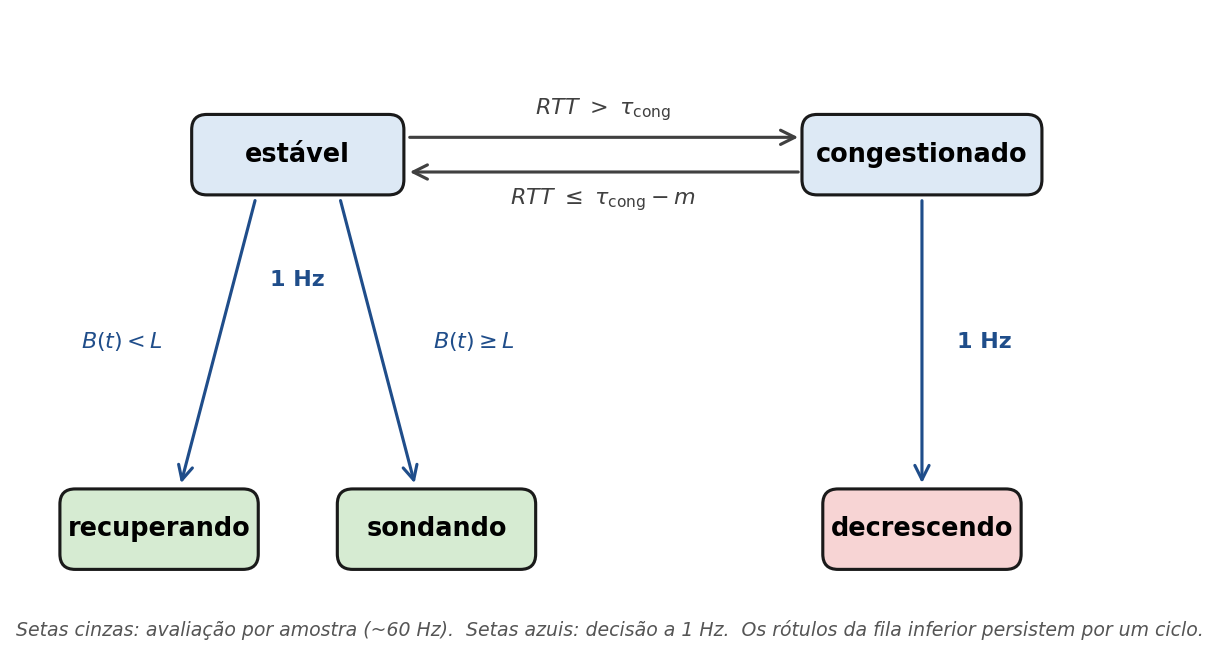
\includegraphics[width=\columnwidth]{images/state_machine.png}
  \caption{Máquina de estados do controlador MACCA. A
  cada amostra de RTT (setas cinzas), o controlador transita
  entre os estados \emph{estável} e \emph{congestionado}
  conforme o RTT ultrapassa o limiar $\tau_{\rm cong}$ ou
  retorna abaixo de $\tau_{\rm cong} - m$, onde $m$ é a margem
  de histerese. A cada ciclo de decisão a 1~Hz (setas azuis),
  e desde que o \emph{streak} de duração mínima associado
  ($h_{\rm down}$ para decrementos, $h_{\rm up}$ para
  incrementos) tenha sido acumulado, o controlador atua sobre
  a taxa de bits-alvo do codificador: \emph{decrescendo} a
  partir de \emph{congestionado}; \emph{recuperando} ou
  \emph{sondando} a partir de \emph{estável}, conforme a
  amostra $B(t)$ da curva cúbica de recuperação esteja abaixo
  ou acima do teto $L$. Os rótulos da fila inferior persistem
  até o próximo ciclo de decisão.}
  \label{fig:state-machine}
\end{figure}

\subsection{Algoritmo}

\subsubsection{Sinal e Detecção}

O controlador recebe, a cada quadro codificado, uma amostra de
RTT proveniente da biblioteca ENet~\cite{enet}. A partir dessa amostra, dois
contadores de duração são mantidos. O primeiro, denominado
\emph{streak} de congestão, registra o início da janela contínua
mais recente em que o RTT permanece acima do limiar de
referência $\tau_{\text{cong}}$; é reiniciado sempre que uma
amostra retorna a valores aceitáveis. O segundo, denominado
\emph{streak} de via livre, registra simetricamente o início da
janela contínua em que o RTT permanece abaixo de
$\tau_{\text{cong}} - m$, onde $m$ é uma margem de histerese
introduzida pela razão discutida adiante. Os dois contadores são
atualizados continuamente, mas não disparam decisões por si só.

\subsubsection{Decremento Multiplicativo com \emph{Fast Convergence}}

Quando o \emph{streak} de congestão atinge uma duração mínima
$h_{\text{down}}$, o controlador aplica uma redução
multiplicativa à taxa atual:
\begin{equation}
  \text{kbps}_{\text{novo}} \gets \max\!\left( \beta \cdot \text{kbps}, \text{kbps}_{\min} \right)
  \label{eq:decrease}
\end{equation}
onde $\beta \in (0,1)$ é o fator de retenção e
$\text{kbps}_{\min}$ é o piso de operação. Adota-se $\beta = 0{,}7$,
valor utilizado no controlador AIMD de referência e mantido
nesta versão para isolar o efeito das demais alterações.

Antes da redução propriamente dita, o teto de recuperação
$L$ (último valor conhecido considerado seguro) é atualizado.
Em condições normais, em que a taxa atual ainda corresponde ao
último patamar estável, $L$ recebe o valor da taxa atual. Em
condições de congestionamento persistente, em que uma nova
redução é disparada antes que o controlador tenha recuperado o
patamar anterior, situação caracterizada por
$\text{kbps} < L$ no instante do disparo, $L$ é atualizado
segundo o mecanismo de fast convergence do
CUBIC:
\begin{equation}
  L \gets \text{kbps} \cdot \frac{1 + \beta}{2}
  \label{eq:fastconv}
\end{equation}
Esse ajuste retira do controlador a expectativa de retornar a
um teto que se mostrou inalcançável, fazendo-o convergir para
uma estimativa progressivamente mais próxima da capacidade
efetiva do canal. Em cenários de constrição prolongada, o
mecanismo evita que a curva de recuperação descrita a seguir
fique perpetuamente apontando para um valor obsoleto.

\subsubsection{Curva de Recuperação Cúbica}

Quando o \emph{streak} de via livre atinge uma duração mínima
$h_{\text{up}}$, o controlador aplica um incremento à taxa
atual. A magnitude do incremento é determinada por uma
amostragem da curva cúbica de recuperação do
CUBIC~\cite{cubic}:
\begin{equation}
  B(t) = C \cdot (t - K)^3 + L
  \label{eq:cubic-controller}
\end{equation}
onde $t$ é o tempo decorrido em segundos desde a última
redução, $L$ é o teto de recuperação definido por
(\ref{eq:fastconv}), $K$ é o tempo nominal de recuperação até
$L$, e $C = (1 - \beta) \cdot L / K^3$. A nova taxa-alvo é
$B(t)$, restrita ao intervalo $[\text{kbps},
\text{kbps}_{\max}]$, de modo que a curva nunca conduz a uma
redução, apenas a manutenção ou crescimento.

A forma de $B(t)$ é a mesma do CUBIC original, descrita no
Capítulo~\ref{sec:referencial}: côncava para $t < K$,
recuperando rapidamente em direção a $L$; aproximadamente
estável próximo de $t = K$; e convexa para $t > K$, sondando
de forma cautelosa, e depois acelerada, taxas acima do último
patamar conhecido. Para o presente trabalho, adotou-se
$K = 15$~s, valor calibrado empiricamente para que a fase de
sondagem inicie em uma escala compatível com a duração típica
de janelas de constrição nos cenários avaliados.

Variações na ancoragem temporal de $t$ e na regra de reinício do
\emph{streak} de via livre após crescimentos foram avaliadas
empiricamente, com resultados que motivam a forma adotada aqui;
essa análise é apresentada no
Capítulo~\ref{sec:resultados}, Seção~\ref{sec:sensibilidade}.

% [SUGESTÃO DE FIGURA] curva B(t) plotada para K=5s e K=15s
\begin{figure}[!t]
  \centering
  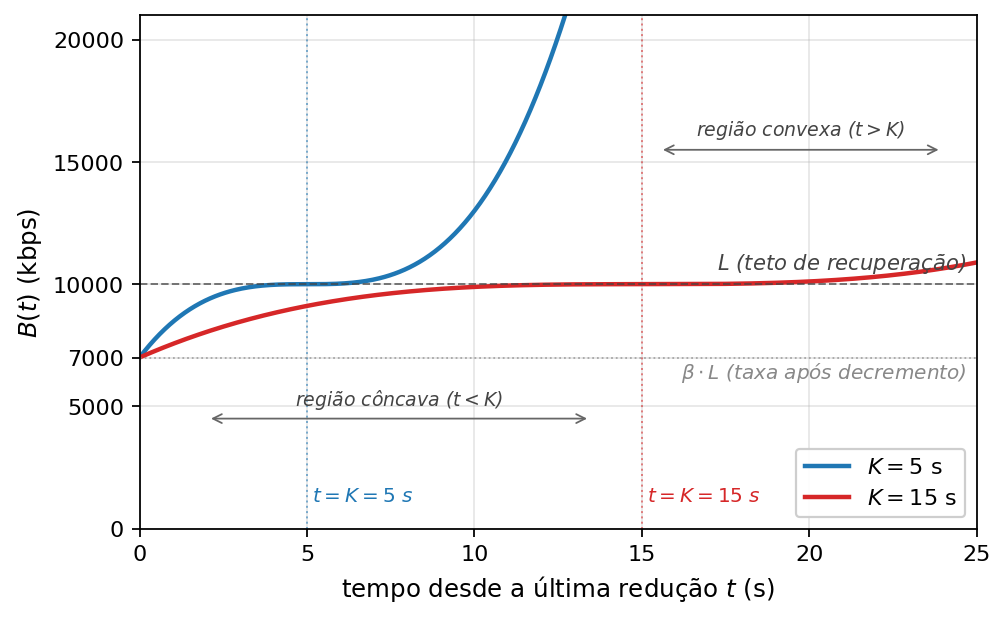
\includegraphics[width=\columnwidth]{images/cubic_curve.png}
  \caption{Curva de recuperação $B(t)$ amostrada pelo
  controlador MACCA para dois valores do parâmetro $K$
  (\SI{5}{\second} e \SI{15}{\second}), com $\beta = 0{,}7$ e
  $L = 10\,000$~kbps. A região côncava ($t < K$) promove
  recuperação rápida em direção ao teto $L$; a região convexa
  ($t > K$) realiza sondagem cautelosa de capacidade adicional.}
  \label{fig:cubic-curve}
\end{figure}

\subsection{Cadência de Decisão e Histerese}

Duas decisões de projeto merecem justificativa explícita por
afetarem diretamente o comportamento dinâmico do controlador: a
cadência de avaliação a 1~Hz e o uso de histerese nos disparos
de decremento e incremento.

A cadência de 1~Hz é menor que a taxa de quadros do codificador
(tipicamente 60~Hz) por escolha deliberada. Reconfigurações
sucessivas e próximas no tempo da taxa do codificador
introduzem custos que vão da reinicialização de contextos
internos do \emph{encoder} ao envio de quadros IDR não
planejados, ambos potencialmente capazes de agravar a própria
condição de congestionamento que o controlador busca aliviar.
Espaçar as decisões em intervalos de um segundo permite que
cada atuação se propague pelo \emph{buffer} do gargalo e
manifeste seu efeito no RTT antes que a próxima decisão seja
tomada, evitando ciclos de realimentação curtos.

A histerese é um mecanismo clássico em sistemas de controle utilizado para evitar oscilações em torno de um limiar de decisão. No controlador proposto, ela é introduzida em dois níveis. Primeiro, exige-se que a condição de disparo (RTT sustentadamente acima ou abaixo do limiar) persista por uma duração mínima --- $h_{\text{down}}$ para decrementos e $h_{\text{up}}$ para incrementos --- antes que qualquer atuação ocorra. Esse requisito filtra picos transitórios de RTT, comuns em redes domésticas, que sob um critério instantâneo poderiam provocar uma sequência indesejada de cortes e recuperações.

Além disso, o controlador utiliza limiares distintos para identificar congestionamento e recuperação. Enquanto a entrada em congestionamento é caracterizada por RTT acima de $\tau_{\text{cong}}$, a condição de via livre exige que o RTT permaneça abaixo de $\tau_{\text{cong}}-m$, onde $m$ é uma margem de histerese. Dessa forma, pequenas oscilações do RTT em torno do limiar não fazem o controlador alternar continuamente entre os dois estados, permitindo que variações compatíveis com o ruído natural da rede sejam absorvidas sem disparar atuações desnecessárias.


Os valores adotados para todos os parâmetros do controlador são
sintetizados na Tabela~\ref{tab:params}. A escolha de cada
valor seguiu a calibração empírica conduzida ao longo do
desenvolvimento e descrita parcialmente no
Capítulo~\ref{sec:metodologia}.

\begin{table}[!t]
  \caption{Parâmetros do controlador MACCA adotados na
  campanha experimental.}
  \label{tab:params}
  \centering
  \begin{tabular}{lll}
    \toprule
    \textbf{Parâmetro} & \textbf{Símbolo} & \textbf{Valor} \\
    \midrule
    Limiar de RTT (congestionamento) & $\tau_{\text{cong}}$ & \SI{100}{\milli\second} \\
    Margem de histerese & $m$ & \SI{20}{\milli\second} \\
    Histerese de decremento & $h_{\text{down}}$ & \SI{2000}{\milli\second} \\
    Histerese de incremento & $h_{\text{up}}$ & \SI{1000}{\milli\second} \\
    Fator de retenção & $\beta$ & 0{,}70 \\
    Tempo nominal de recuperação & $K$ & \SI{15}{\second} \\
    \emph{Fast convergence} & --- & ativo \\
    Intervalo de decisão & --- & \SI{1000}{\milli\second} \\
    Taxa mínima & $\text{kbps}_{\min}$ & \SI{1000}{\kilo\bit\per\second} \\
    Taxa máxima & $\text{kbps}_{\max}$ & inicial da sessão \\
    \bottomrule
  \end{tabular}
\end{table}

\subsection{Integração no Sunshine}

A política de controle foi implementada como uma classe
isolada em \texttt{src/bitrate\_controller.\{h,cpp\}}, contendo
exclusivamente lógica de decisão, sem qualquer acoplamento a
mecanismos de entrada ou saída do servidor. A classe expõe um
único método de atualização, \texttt{on\_sample}, que recebe
uma estrutura com a amostra de RTT corrente e retorna,
opcionalmente, uma nova taxa de bits-alvo quando uma decisão
de atuação é tomada. Essa separação preserva a testabilidade
do componente, viabilizando cobertura por testes unitários em
\emph{gtest}~\cite{gtest} sob \texttt{tests/} sem necessidade de
infraestrutura de rede.

A integração com o restante do servidor ocorre em
\texttt{src/stream.cpp}, no laço principal de transmissão de
vídeo. A cada quadro codificado, a \emph{thread} de
\emph{broadcast} consulta o RTT corrente fornecido pela
biblioteca ENet e invoca \texttt{on\_sample}; quando o
controlador retorna uma nova taxa-alvo, a \emph{thread} aciona
o mecanismo de reconfiguração do codificador.

Os parâmetros do controlador foram expostos ao usuário em
\texttt{src/config.cpp}, junto aos demais parâmetros de
\emph{streaming}. A escolha de tornar os parâmetros
configuráveis, em vez de fixá-los no código, decorre da
expectativa de que diferentes perfis de uso, tipos de jogo e
condições típicas de rede do usuário possam exigir calibrações
próprias, e do reconhecimento de que a campanha
experimental conduzida neste trabalho cobre apenas um
subconjunto desses cenários. As mensagens visíveis ao usuário
adotam \texttt{boost::locale::translate} para internacionalização,
em conformidade com a convenção do projeto. O código segue as
diretrizes de formatação do \texttt{.clang-format} do
repositório e foi submetido como contribuição ao projeto
\emph{upstream}.


\section{Metodologia}\label{sec:metodologia}

Este capítulo apresenta o ambiente experimental e os procedimentos utilizados para avaliar o controlador proposto.

\subsection{Testbed e Carga de Trabalho}

O servidor de \emph{streaming} executa o Sunshine sobre o
hardware descrito na Tabela~\ref{tab:testbed}.

\begin{table}[!t]
  \caption{Especificações do testbed experimental.}
  \label{tab:testbed}
  \centering
  \begin{tabular}{ll}
    \toprule
    \textbf{Componente} & \textbf{Especificação} \\
    \midrule
    CPU (servidor) & AMD Ryzen 7 7700 (8 núcleos, 16 \emph{threads}) \\
    RAM (servidor) & 32~GB \\
    GPU (servidor) & NVIDIA GeForce RTX 4070 SUPER \\
    Codificador & NVENC \\
    Sistema operacional & Fedora Linux 43 \\
    \emph{Kernel} & Linux 6.19 \\
    Interface de rede (servidor) & Ethernet 1~Gbps \\
    Cliente & Smartphone Android, \emph{Moonlight} \\
    Conexão do cliente & Wi-Fi, mesma rede local \\
    \bottomrule
  \end{tabular}
\end{table}

A degradação de rede foi emulada no servidor via \texttt{tc}~\cite{iproute2}
com disciplina HTB, aplicada à interface de saída \texttt{eno1}.
Essa abordagem permite limitar a capacidade do enlace de forma
determinística e reproduzível, sem introduzir atrasos
artificiais que poderiam confundir o sinal de RTT utilizado
pelo controlador. Os \emph{scripts} de \emph{shaping} adotados estão disponíveis
no repositório do projeto.

A carga de trabalho utilizada em todas as sessões foi o jogo
\emph{Celeste}, escolhido por três motivos complementares. O
primeiro é o perfil de \emph{rendering} leve: o estilo
visual 2D mantém a taxa de bits demandada pelo codificador em
patamares relativamente estáveis, evitando que a variação do
canal seja confundida com variação do conteúdo. O segundo é a
sensibilidade do \emph{gameplay} à latência: a mecânica
baseia-se em saltos de precisão e janelas curtas de reação,
condição em que travamentos e atrasos são imediatamente
perceptíveis ao operador. O terceiro é a previsibilidade do
comportamento entre sessões, característica desejável para que
diferenças observadas entre controladores possam ser atribuídas
ao próprio controlador, e não ao conteúdo exibido. 

\subsection{Cenários de Avaliação}

Foram definidos seis cenários de degradação de rede,
sintetizados na Tabela~\ref{tab:scenarios}, escolhidos para
cobrir as principais formas em que um canal doméstico pode
degradar ao longo de uma sessão de jogo. Os cenários variam em
três dimensões complementares: a forma da degradação (queda
abrupta, em degraus, em janelas alternadas, ou contínua); a
severidade da constrição (de \SI{16}{\mega\bit\per\second}
até \SI{4}{\mega\bit\per\second}); e a duração total do
período sob shaping (de janelas curtas de \SI{30}{\second} a
constrições contínuas de \SI{160}{\second}). Fora das janelas
indicadas, o enlace opera sem restrição imposta pelo
\texttt{tc}, ou seja, na capacidade nativa de \SI{1}{\giga\bit\per\second}.

\begin{table}[!t]
  \caption{Cenários de degradação de rede utilizados na campanha
  experimental. Fora das janelas indicadas, o canal opera sem
  restrição.}
  \label{tab:scenarios}
  \centering
  \begin{tabular}{cll}
    \toprule
    \textbf{Cenário} & \textbf{Capacidade} & \textbf{Janela de shaping} \\
    \midrule
    A & 8~Mbps & 80--160~s \\
    B & 16 / 12 / 8~Mbps & 60--90 / 90--120 / 120--160~s \\
    C & 14 / 10~Mbps & 40--120 / 120--200~s \\
    D & 10~Mbps & 30--60 / 90--120 / 150--180 / 210--240~s \\
    E & 4~Mbps & 40--200~s \\
    F & 6~Mbps & 0--160~s \\
    \bottomrule
  \end{tabular}
\end{table}

O cenário~A representa uma queda abrupta e prolongada,
testando a capacidade do controlador de reagir a um corte
único e sustentado. O cenário~B aplica degraus sucessivos de
severidade crescente, exigindo do controlador adaptações
encadeadas em curto intervalo. O cenário~C aplica dois
patamares mais longos, simulando uma transição entre regimes
de banda. O cenário~D alterna entre quatro janelas curtas de
constrição e períodos de recuperação, testando o
comportamento do controlador em ciclos de degradação e
restauração. Os cenários~E e~F representam constrições
contínuas, severa e moderada respectivamente, em que o
controlador deve estabilizar a operação dentro do envelope
imposto pela rede.

\subsection{Controladores Comparados}

Três controladores foram avaliados, identificados como
referência fixa, AIMD de base e MACCA. O controlador de
referência fixa corresponde ao comportamento original do
Sunshine, em que a taxa de bits é negociada uma única vez ao
início da sessão e mantida constante até o fim. O controlador
AIMD de base aplica corte multiplicativo com fator $\beta = 0{,}7$
ao detectar congestionamento e cresce em duas fases
(``$\times \gamma$ depois $+\Delta$''), sem o mecanismo de
\emph{fast convergence}; corresponde à versão do controlador
adaptativo que antecedeu a contribuição apresentada neste
trabalho. O controlador MACCA corresponde à contribuição
descrita no Capítulo~\ref{sec:contribuicao}, com os parâmetros
sintetizados na Tabela~\ref{tab:params}.

\subsection{Instrumentação e Métricas}

A coleta de dados em \emph{runtime} é realizada pelo próprio
Sunshine por meio de uma extensão de instrumentação
desenvolvida durante este trabalho. A cada amostra de RTT recebida
da biblioteca ENet, um registro é exportado para um arquivo
CSV contendo o instante de amostragem, o RTT, a variância do
RTT, o tempo de envio do quadro mais recente, o tamanho do
quadro codificado, a taxa de bits-alvo corrente, o estado do
controlador e indicadores de eventos relevantes (envio de
quadro IDR, requisição de IDR pelo cliente). A taxa de
amostragem é a própria taxa de quadros do codificador,
tipicamente próxima de \SI{60}{\hertz}.

A partir do CSV de cada sessão são derivadas as métricas
agregadas reportadas no Capítulo~\ref{sec:resultados}. As
métricas de latência incluem o pico de RTT, os percentis 50,
95 e 99 da distribuição, e a fração do tempo total em que o
RTT excede o limiar de \SI{100}{\milli\second} estabelecido
como referência para jogos de ação~\cite{baldovino2022}. As
métricas de throughput incluem a taxa de bits média sustentada
durante a janela de shaping e o uso do canal, definido como a
razão entre essa média e a capacidade imposta pela emulação.
As métricas de continuidade incluem a contagem de \emph{stalls},
definidos como intervalos consecutivos superiores a
\SI{100}{\milli\second} sem entrega de quadros ao cliente, o
tempo total acumulado em \emph{stall}, e a contagem de quadros
IDR emitidos durante a sessão. Esta última é utilizada como
indicador indireto de recuperação após perdas que escaparam aos
mecanismos de FEC.

Adicionalmente, ao final de cada sessão o operador registrou
três avaliações subjetivas em escala de 1 a 5, em que 1
corresponde à melhor avaliação: \emph{latência percebida},
\emph{qualidade visual} e \emph{estabilidade}.

\subsection{Protocolo de Execução}

A campanha experimental do controlador MACCA compreendeu uma execução para cada combinação de controlador e cenário, totalizando seis novas execuções. Os resultados correspondentes aos controladores fixo e AIMD de base foram reaproveitados de uma campanha anterior realizada sobre o mesmo \emph{testbed} e com a mesma configuração do servidor, em razão da baixa variabilidade observada entre repetições.

Em todas as execuções, o jogo \emph{Celeste} foi utilizado como carga de trabalho, seguindo uma sequência de fases pré-determinada com duração aproximada de quatro minutos. O tráfego do enlace foi submetido aos cenários de \emph{shaping} descritos na Tabela~\ref{tab:scenarios}, iniciados no instante zero da sessão. Ao término de cada execução, foram registradas as avaliações subjetivas descritas na seção anterior, e os dados exportados pelo Sunshine foram armazenados para posterior análise.

\subsection{Uso de Inteligência Artificial como Ferramenta de Pesquisa}

Ferramentas de inteligência artificial baseadas em LLM foram empregadas em dois pontos do
trabalho. O primeiro foi o apoio à implementação em C++ do
controlador e de sua integração ao Sunshine, incluindo o
ajuste de testes em \emph{gtest} e a conformidade com as
convenções de estilo do projeto \emph{upstream}. Todo o código
produzido com esse apoio foi revisado, compilado e testado pelo
pesquisador antes de qualquer submissão ao repositório
\emph{upstream}, e nenhuma alteração foi incorporada sem
verificação.

O segundo foi a estruturação de uma base de conhecimento
local, em formato Markdown compatível com o \emph{Obsidian},
utilizada como apoio à navegação do material bibliográfico, da
documentação interna do Sunshine, e do registro das iterações
de \emph{design} do controlador. A base é composta por
análises individuais (de \emph{papers} lidos, de subsistemas
do Sunshine e de Linux, e de cada iteração de projeto), com
referências cruzadas via \emph{wikilinks} que permitem
visualização em grafo. A síntese inicial de cada arquivo foi
auxiliada por IA a partir da leitura primária do material pelo
pesquisador, com edições e validações subsequentes realizadas
manualmente.

O uso de IA neste trabalho restringiu-se ao apoio à
implementação de código e à estruturação da base de
conhecimento de pesquisa, ambos sob revisão e validação do
pesquisador. As decisões de projeto, a análise dos resultados
experimentais e as conclusões apresentadas são de autoria
própria.

\section{Resultados}\label{sec:resultados}

\subsection{Visão Geral}

A Tabela~\ref{tab:results-full} sintetiza, para cada par
(controlador, cenário), as métricas agregadas definidas no
Capítulo~\ref{sec:metodologia}. A Figura~\ref{fig:summary-bars}
visualiza as principais delas em forma comparativa.

\begin{table*}[!t]
  \caption{Resultados agregados da campanha experimental.
  Valores em negrito indicam o melhor desempenho entre os três
  controladores no respectivo cenário; as colunas de
  decrementos, incrementos e quadros IDR registram atividade do
  controlador e não admitem ordenação direta. Para as
  avaliações subjetivas (escala 1~=~melhor, 5~=~pior), o
  destaque marca o controlador subjetivamente preferido,
  conforme menor soma das três notas.}
  \label{tab:results-full}
  \centering
  \footnotesize
  \begin{tabular}{cl rrrr rr rr r c}
    \toprule
    \textbf{Cenário} & \textbf{Controlador} &
    \textbf{Pico} & \textbf{p99} & \textbf{p95} & \textbf{p50} &
    \textbf{Decr.} & \textbf{Incr.} &
    \textbf{Stalls} & \textbf{T. stall} & \textbf{IDR} &
    \textbf{lat/qual/estab} \\
    & & (ms) & (ms) & (ms) & (ms) & & & & (ms) & & \\
    \midrule
    \multirow{3}{*}{A} & sem ABR     & 1854 & 1801 & 1723 & \textbf{4} & 0 & 0 & 43 & 49\,337 & 10 & 5 / 1 / 5 \\
                      & AIMD de base & 1786 & 1713 & \textbf{55} & \textbf{4} & 7 & 25 & 4 & 4408 & 35 & \textbf{3 / 1 / 3} \\
                      & MACCA   & \textbf{1025} & \textbf{913} & 183 & 16 & 9 & 82 & \textbf{0} & \textbf{0} & 97 & 3 / 2 / 3 \\
    \midrule
    \multirow{3}{*}{B} & sem ABR     & 1551 & 1481 & 1323 & \textbf{5} & 0 & 0 & 50 & 43\,550 & 27 & 4 / 1 / 4 \\
                      & AIMD de base & 575 & 544 & 194 & \textbf{4} & 7 & 22 & \textbf{0} & \textbf{0} & 30 & \textbf{1 / 1 / 2} \\
                      & MACCA   & \textbf{532} & \textbf{486} & \textbf{123} & 18 & 7 & 67 & \textbf{0} & \textbf{0} & 78 & 3 / 2 / 2 \\
    \midrule
    \multirow{3}{*}{C} & sem ABR     & 1565 & 1541 & 1481 & \textbf{6} & 0 & 0 & 107 & 87\,452 & 104 & 4 / 1 / 4 \\
                      & AIMD de base & 733 & \textbf{504} & \textbf{116} & \textbf{5} & 7 & 28 & \textbf{0} & \textbf{0} & 36 & \textbf{1 / 1 / 1} \\
                      & MACCA   & \textbf{639} & 566 & 298 & 13 & 12 & 115 & \textbf{0} & \textbf{0} & 133 & 2 / 1 / 3 \\
    \midrule
    \multirow{3}{*}{D} & sem ABR     & 1583 & 1531 & 1442 & 16 & 0 & 0 & 103 & 91\,501 & 97 & 4 / 1 / 3 \\
                      & AIMD de base & 1156 & \textbf{877} & \textbf{117} & \textbf{5} & 7 & 31 & \textbf{0} & \textbf{0} & 39 & \textbf{2 / 1 / 2} \\
                      & MACCA   & \textbf{998} & 979 & 522 & 12 & 16 & 161 & \textbf{0} & \textbf{0} & 186 & 3 / 1 / 3 \\
    \midrule
    \multirow{3}{*}{E} & sem ABR     & 3788 & 3630 & 3435 & 22 & 0 & 0 & 59 & 135\,167 & 5 & 5 / 1 / 5 \\
                      & AIMD de base & 3808 & 3533 & 3354 & \textbf{5} & 16 & 25 & 5 & 11\,010 & 43 & 3 / 3 / 3 \\
                      & MACCA   & \textbf{3311} & \textbf{3185} & \textbf{2980} & 23 & 16 & 128 & \textbf{2} & \textbf{4306} & 151 & 3 / 3 / 4 \\
    \midrule
    \multirow{3}{*}{F} & sem ABR     & 2536 & 2453 & 2308 & 22 & 0 & 0 & 100 & 148\,855 & 72 & 5 / 1 / 4 \\
                      & AIMD de base & \textbf{1602} & \textbf{1551} & \textbf{263} & \textbf{5} & 13 & 33 & \textbf{2} & \textbf{2852} & 50 & 3 / 2 / 3 \\
                      & MACCA   & 1863 & 1832 & 477 & 12 & 17 & 128 & 4 & 5961 & 156 & \textbf{2 / 1 / 2} \\
    \bottomrule
  \end{tabular}
\end{table*}

\begin{figure*}[!t]
  \centering
  \includegraphics[width=\textwidth]{images/summary_bars.png}
  \caption{Comparação entre os três controladores nos seis
  cenários, agrupada por métrica. Da esquerda para a direita:
  pico de RTT, percentil 99, percentil 95, tempo total
  acumulado em \emph{stall}, e contagem de quadros IDR
  emitidos.}
  \label{fig:summary-bars}
\end{figure*}

Três observações orientam a discussão subsequente. Primeiro, o
controlador MACCA apresenta o menor pico de RTT em cinco
dos seis cenários (A, B, C, D, E), com a maior redução
ocorrendo no cenário~A (1786 para 1025~ms, queda de 43\%).
Segundo, o mesmo controlador eleva o RTT mediano (p50) em
todos os cenários, passando de 4--5~ms no controlador AIMD de
base para 12--23~ms no MACCA. Terceiro, a comparação com
a referência sem ABR é categórica: o tempo total acumulado em
\emph{stall} cai entre 90\% e 100\% nos dois controladores
adaptativos relativamente ao caso sem controle, com
\SI{40}{\second}--\SI{150}{\second} de \emph{stall} por sessão
de quatro minutos no controlador fixo. A ausência de ABR é
consistentemente a pior experiência, independentemente da
forma da degradação.

\subsection{Análise por Cenário}

A análise cenário a cenário esclarece em quais regimes cada
controlador opera melhor. A Figura~\ref{fig:timelines} reúne
as trajetórias de RTT ao longo das sessões, com o perfil de
\emph{shaping} sobreposto como referência visual.

\begin{figure*}[!t]
  \centering
\includegraphics[width=\textwidth,height=0.75\textheight,keepaspectratio]{images/timelines.png}   \caption{Trajetórias de RTT ao longo das sessões nos seis
  cenários, para cada controlador. As regiões sombreadas
  indicam as janelas de \emph{shaping} ativas. A escala de
  tempo é a duração da sessão (~\SI{240}{\second}); a escala de
  RTT é logarítmica para preservar a visibilidade simultânea
  do regime estacionário e dos picos.}
  \label{fig:timelines}
\end{figure*}

\textbf{Cenário A (queda abrupta).} A queda súbita de banda
livre para \SI{8}{\mega\bit\per\second} em $t=\SI{80}{\second}$
expõe o ganho mais nítido do controlador MACCA. O pico de
RTT cai 43\% em relação ao AIMD de base (1025 \emph{vs.}
1786~ms), e o número de \emph{stalls} é reduzido a zero. A
combinação da curva cúbica de recuperação com o mecanismo de
\emph{fast convergence} absorve a restrição sem que o
codificador chegue a congelar. O controlador AIMD de base,
ainda que apresente p95 substancialmente menor (55 \emph{vs.}
183~ms), exibe um pico de cauda próximo do observado sem ABR.

\textbf{Cenário B (degraus sucessivos).} A redução gradual em
três degraus (16~/~12~/~8~Mbps) é o cenário em que o
controlador AIMD de base mais se beneficia de sua simplicidade.
A diferença no pico de RTT entre os dois controladores
adaptativos é pequena (575 \emph{vs.} 532~ms, queda de 7\% no
MACCA). O regime estacionário, porém, é claramente
superior no AIMD de base, com p50 de 4~ms contra 18~ms do AIMD
CUBIC, e essa vantagem se reflete na avaliação subjetiva
amplamente favorável (1~/~1~/~2 \emph{vs.} 3~/~2~/~2). O p95
do MACCA (123~ms) é, contudo, menor que o do AIMD de base
(194~ms), indicando que a contenção de picos isolados ocorre
mesmo nesse cenário em que o regime estacionário é a dimensão
dominante da percepção.

\textbf{Cenário C (dois patamares).} A transição lenta entre
14 e \SI{10}{\mega\bit\per\second} expõe um padrão similar ao
do cenário~B. O MACCA reduz o pico em 13\%, mas o AIMD
de base alcança a única avaliação subjetiva perfeita da
campanha (1~/~1~/~1). O p95 do MACCA (298~ms) é mais que
o dobro do AIMD de base (116~ms), e essa elevação do regime
estacionário é percebida pelo operador como degradação visual
ainda que os eventos de cauda sejam menos frequentes.

\textbf{Cenário D (janelas curtas alternadas).} O padrão de
quatro janelas de \SI{30}{\second} de constrição alternadas
com períodos livres é o que mais desafia o MACCA. A cada
janela livre, o controlador inicia uma sondagem cúbica
agressiva; a cada nova constrição, dispara uma cascata de
cortes. O resultado é um p95 explodido (522 \emph{vs.} 117~ms
do AIMD de base) e uma sensação de instabilidade,
caracterizada pelas 161 atuações de incremento ao longo da
sessão. O pico de RTT é levemente menor no MACCA (998
\emph{vs.} 1156~ms), mas a vantagem é eclipsada pela piora
do regime estacionário.

\textbf{Cenário E (constrição pesada longa).} A restrição
para \SI{4}{\mega\bit\per\second} sustentada por
\SI{160}{\second} é o cenário mais severo da campanha, e
aquele em que o argumento favorável ao MACCA se
sustenta com maior força. O pico de RTT cai de 3808 para
3311~ms (13\%), e o tempo total em \emph{stall} é reduzido de
\SI{11.0}{\second} para \SI{4.3}{\second}, queda de 61\%. O
controlador sem ABR sofre \SI{135}{\second} de \emph{stall}
acumulado sobre os \SI{160}{\second} de constrição, equivalente
a 84\% do período: do ponto de vista do jogador, a sessão é
efetivamente tornada injogável.

\textbf{Cenário F (constrição moderada contínua).} A
restrição para \SI{6}{\mega\bit\per\second} ativa desde
$t=0$ é o único cenário em que o MACCA regride
relativamente ao AIMD de base. O pico de RTT sobe 16\%
(1602 para 1863~ms) e o tempo em \emph{stall} é mais que
dobrado. O diagnóstico é estrutural: como a constrição existe
desde o início da sessão, o controlador nunca chega a operar
em uma fase não restrita; o teto de recuperação
\texttt{last\_known\_good} é inicializado com o valor
negociado de sessão (próximo de \SI{19}{\mega\bit\per\second})
e a curva inicial de recuperação fica apontada para esse teto
fictício, jamais alcançável. O mecanismo de \emph{fast
convergence} corrige progressivamente o teto à medida que
cascatas sucessivas ocorrem, mas a primeira janela de
recuperação é desperdiçada buscando uma capacidade que nunca
esteve disponível. Vale notar, contudo, que a avaliação
subjetiva no cenário~F favorece o MACCA (2~/~1~/~2
\emph{vs.} 3~/~2~/~3 do AIMD de base), evidenciando que pico
de RTT e percepção subjetiva não se alinham de forma
mecânica.

\subsection{Trade-off entre Métricas de Cauda e de Regime Estacionário}

A análise conjunta dos resultados revela um trade-off sistemático entre métricas de cauda da distribuição de latência (pico, p99 e eventos de \emph{stall}) e métricas do regime estacionário (mediana e percentis intermediários). A Figura~\ref{fig:tradeoff-scatter} sintetiza esse comportamento em uma única representação.

\begin{figure}[!t]
\centering
\includegraphics[width=\columnwidth]{images/tradeoff_scatter.png}
\caption{Trade-off entre pico de RTT (cauda) e mediana de RTT (regime estacionário). Cada ponto representa um par (controlador, cenário). Eixos em escala logarítmica. O canto inferior-esquerdo representa o ideal.}
\label{fig:tradeoff-scatter}
\end{figure}

O agrupamento dos pontos por controlador é nítido. O AIMD de base concentra-se em medianas próximas de 4--5~ms, mas apresenta picos que cobrem praticamente todo o eixo vertical, alcançando valores superiores a \SI{3.5}{\second} no cenário~E. O MACCA, por sua vez, opera com medianas mais elevadas (12--23~ms), porém limita de forma mais consistente os eventos de cauda. Nenhum dos dois controladores domina o outro simultaneamente nos dois eixos, de modo que ambos contribuem para a fronteira de Pareto observada.

A Figura~\ref{fig:rtt-cdf} reforça essa interpretação ao apresentar as distribuições cumulativas empíricas do RTT. As curvas do AIMD de base concentram grande parte das amostras em RTTs baixos, mas exibem caudas mais longas. Já o MACCA apresenta um piso mais elevado, porém com menor dispersão dos valores extremos. Em todos os cenários, as curvas dos dois controladores cruzam-se em torno de \SI{100}{\milli\second}.

\begin{figure*}[!t]
\centering
\includegraphics[width=\textwidth]{images/rtt_cdf_panel.png}
\caption{Distribuição cumulativa empírica (CDF) do RTT por cenário e por controlador. A linha pontilhada marca o limiar de \SI{100}{\milli\second}.}
\label{fig:rtt-cdf}
\end{figure*}

Em síntese, o MACCA privilegia a contenção dos eventos extremos ao custo de uma elevação do RTT típico, enquanto o AIMD de base favorece o regime estacionário em detrimento de menor proteção contra picos de latência. A escolha entre ambos corresponde, portanto, a uma decisão de projeto sobre qual região da distribuição se deseja priorizar, e não a um juízo absoluto sobre qualidade.


\subsection{Análise de Sensibilidade ao Design da Curva}\label{sec:sensibilidade}

A curva de recuperação cúbica adotada na contribuição
(Capítulo~\ref{sec:contribuicao}) foi escolhida após avaliação
empírica de duas variantes alternativas, ambas mais fiéis à
formulação original do algoritmo CUBIC~\cite{cubic}. A primeira
variante, identificada como~5b, ancora o tempo decorrido $t$ da
curva no instante de retorno do RTT à condição de via livre
(\texttt{rtt\_clear\_since}) em vez do instante da última redução
(\texttt{last\_decrease\_at}). A motivação era teórica: o $t-K$
da curva pretende medir o tempo desde que o canal está
genuinamente livre, e \texttt{rtt\_clear\_since} captura isso
melhor que \texttt{last\_decrease\_at}, contaminado pelo
tempo de drenagem do \emph{buffer}. A segunda variante,
identificada como~5c, mantém a âncora em
\texttt{last\_decrease\_at} mas deixa de reinicializar o
\emph{streak} de via livre após cada incremento bem-sucedido,
permitindo que $t$ acumule monotonicamente entre cortes. Essa
é a interpretação literal do parágrafo §3.1 do trabalho
original do CUBIC.

A Tabela~\ref{tab:sensitivity} apresenta o pico de RTT obtido
em sessões repetidas dos cenários~A e~E com cada variante,
mantidos os demais parâmetros.

\begin{table}[!t]
  \caption{Pico de RTT (em ms) sob três variantes de design da
  curva de recuperação. A forma final é a adotada na
  contribuição. Variantes regrediram em todos os casos
  avaliados.}
  \label{tab:sensitivity}
  \centering
  \begin{tabular}{lrrr}
    \toprule
    \textbf{Variante} & \textbf{A K=5\,s} & \textbf{A K=15\,s} & \textbf{E K=15\,s} \\
    \midrule
    Forma final (Idea 5)  & 796   & 1221  & \textbf{2305} \\
    Variante 5b           & 1105 \scriptsize($+39\%$) & 1313 \scriptsize($+8\%$)  & 3192 \scriptsize($+39\%$) \\
    Variante 5c           & 1116 \scriptsize($+40\%$) & 1264 \scriptsize($+4\%$)  & 3013 \scriptsize($+31\%$) \\
    \bottomrule
  \end{tabular}
\end{table}

A regressão é sistemática nos cenários constrangidos,
particularmente no cenário~E, em que ambas as variantes
elevam o pico em mais de 30\% relativamente à forma final. O
diagnóstico é estrutural. A curva cúbica do CUBIC original foi
formulada para amostragem por~ACK, regime em que cada
atualização da janela aplica um delta pequeno acumulado ao
longo de muitas iterações por segundo. No controlador aqui
proposto, a curva é amostrada a uma cadência de 1~Hz, em que
cada atualização aplica o delta integral entre dois instantes
de decisão. As variantes mais fiéis ao paper original mostram
\emph{overshoot} sistemático: o controlador cresce mais do que
o canal pode absorver, dispara congestionamento novamente, e
permanece em ciclo. A variante final, ao reinicializar
o \emph{streak} de via livre após cada crescimento, impõe um
intervalo mínimo de espera entre crescimentos sucessivos, o
que funciona como uma forma implícita de filtragem temporal
ausente na formulação original.

Esse achado tem alcance maior que a presente contribuição.
Algoritmos de controle de congestionamento projetados para
amostragem densa não são, em geral, transponíveis a regimes de
cadência reduzida sem ajuste estrutural. No caso do CUBIC, a
adaptação que se mostrou empiricamente superior é também a
mais simples, contradizendo a intuição de que maior fidelidade
ao paper original implicaria melhor desempenho.

\subsection{Avaliação Subjetiva}

A Figura~\ref{fig:ratings} apresenta as três avaliações
subjetivas registradas ao final de cada sessão.

\begin{figure*}[!t]
  \centering
  \includegraphics[width=\textwidth]{images/ratings.png}
  \caption{Avaliações subjetivas (escala 1~=~melhor,
  5~=~pior) por cenário e por controlador, organizadas em
  três eixos: latência percebida, qualidade visual e
  estabilidade.}
  \label{fig:ratings}
\end{figure*}

A avaliação subjetiva contradiz parcialmente a ordenação
sugerida pelas métricas de cauda. O controlador AIMD de base
recebe avaliações estritamente melhores nos cenários~B, C e~D,
apesar de seu pico de RTT ser igual ou pior que o do AIMD
CUBIC nesses mesmos cenários. O MACCA, por sua vez,
recebe avaliação subjetiva claramente superior no cenário~F,
em que perde nos picos de RTT. Nos cenários~A e~E as
avaliações são próximas. A leitura natural é que o regime
estacionário (refletido em p50 e p95) tem peso perceptual
maior que eventos de cauda isolados, exceto quando esses
eventos ocorrem em magnitude e frequência elevadas, como no
cenário~E.

Esse padrão alinha-se às observações de QoE em jogos em
nuvem discutidas no Capítulo~\ref{sec:referencial}: a
percepção do usuário é mais sensível à constância do que ao
pico absoluto, contanto que o pico permaneça abaixo de um
limiar de tolerância. Quando esse limiar é ultrapassado, como
no cenário~E, a avaliação subjetiva se aproxima à medida que
o desempenho objetivo se distingue.

\section{Conclusão}\label{sec:conclusao}

Este trabalho propôs e avaliou o MACCA, um
controlador adaptativo de taxa de bits para o servidor de
\emph{streaming} de jogos em nuvem Sunshine. O controlador
estende um esquema AIMD com duas primitivas do algoritmo
CUBIC~\cite{cubic}, a curva cúbica de recuperação após
reduções e o mecanismo de \emph{fast convergence}, e opera
exclusivamente a partir do RTT mantido pela biblioteca ENet
no canal de controle, sem qualquer cooperação adicional do
cliente. Avaliado contra um controlador de referência fixa e
uma variante AIMD de base ao longo de seis cenários de
degradação de rede, o controlador proposto reduz o pico de
RTT em cinco dos seis cenários, com a maior queda alcançando
43\% no cenário~A, e o tempo total acumulado em \emph{stall}
em cinco dos seis cenários, com queda de 61\% no cenário~E.
Esses ganhos são acompanhados de uma elevação sistemática do
RTT mediano, de 4--5~ms no AIMD de base para 12--23~ms no
MACCA, configurando um trade-off explícito entre
desempenho na cauda da distribuição de latência e desempenho
no regime estacionário. Os dois controladores representam,
portanto, escolhas de prioridade complementares, não soluções
mutuamente dominantes.

\subsection{Achados que Transcendem o Sunshine}

A análise de sensibilidade ao design da curva (§\ref{sec:sensibilidade})
isolou um achado de alcance maior que a contribuição
imediata. Variantes mais fiéis à formulação original do CUBIC,
incluindo a interpretação literal do parágrafo §3.1 do
trabalho original, mostraram-se sistematicamente inferiores à
forma final adotada neste trabalho. O diagnóstico é
estrutural: a curva cúbica do CUBIC foi formulada para
amostragem por~ACK, regime em que pequenos deltas se acumulam
ao longo de muitas iterações por segundo. Em controladores
amostrados a cadências reduzidas, como o aqui proposto em
1~Hz, a curva passa a aplicar o delta integral entre instantes
de decisão, e a fidelidade ao paper original deixa de ser
empiricamente desejável. A transposição de algoritmos de
controle de congestionamento entre regimes de cadência exige,
portanto, ajuste estrutural, não apenas reparametrização.

Dois outros achados merecem destaque. O primeiro é que o RTT
mantido server-side pela biblioteca ENet é, isoladamente,
sinal suficiente para um controlador útil em jogos em nuvem,
sem que sejam necessárias extensões de protocolo nem
sincronização de relógio entre cliente e servidor. O segundo é
que métricas de cauda (pico, percentil~99, eventos de
\emph{stall}) e métricas centrais (mediana, percentis
intermediários) devem ser reportadas conjuntamente para
caracterização correta de controladores adaptativos: nenhuma
das duas isoladamente é suficiente para distinguir prioridades
de projeto, e o desempenho subjetivo correlaciona de forma
não-trivial com ambas.

\subsection{Trabalhos Futuros}

Cinco direções concretas emergem como continuação natural
deste trabalho. A primeira é a introdução de uma memória de
capacidade efetiva entre sessões, motivada pela regressão
observada no cenário~F. Naquele cenário, a curva inicial de
recuperação fica apontada para o teto negociado de sessão,
inalcançável dada a constrição ativa desde $t=0$. Uma
estimativa de capacidade carregada da sessão anterior
permitiria que o controlador iniciasse com um teto
\texttt{last\_known\_good} mais próximo da capacidade real do
caminho, evitando a primeira cascata desperdiçada.

A segunda direção é a adoção de um sinal de detecção
sub-segundo, possivelmente a partir do tempo de envio do
quadro mais recente (\texttt{frame\_send\_ms}, já coletado na
instrumentação atual). A latência de reação do controlador
proposto é da ordem da histerese de decremento, e um sinal
adicional que se manifeste antes da inflação do RTT pode
encurtar o tempo entre o início do congestionamento e o corte
de taxa.

A terceira direção é a introdução de um gatilho preditivo
baseado em gradiente, na linha do controlador GCC para
WebRTC~\cite{gcc}, capaz de antecipar a transição da fase de
não-congestionamento para a fase de enfileiramento antes que
o RTT cruze o limiar.

A quarta direção é a condução de uma avaliação subjetiva
\emph{crowdsourced}, segundo o protocolo de Hong et
al.~\cite{hong2015}, em substituição às avaliações de
operador único conduzidas neste trabalho. Esse formato
permite quantificação estatística de Mean Opinion Score sob
diferentes perfis de jogador, tipos de jogo, e condições de
rede.

A quinta direção é a comparação direta do MACCA contra o
GCC~\cite{gcc} e o ABRAGame~\cite{abragame} em um mesmo
testbed, com a mesma instrumentação. Embora os trabalhos
correlatos tenham reportado seu desempenho em ambientes
próprios, a comparação cruzada em ambiente comum é a única
forma robusta de posicionar o presente trabalho contra o
estado da arte em métricas absolutas.

\subsection{Impacto}

O controlador proposto, juntamente com a instrumentação de
coleta de métricas que o sustenta, será submetido como
contribuição ao repositório \emph{upstream} do Sunshine sob a
licença GPL-3.0 do projeto. O testbed experimental, os
\emph{scripts} de geração de cenários, os dados de cada
sessão e os \emph{notebooks} de análise estão disponíveis para
reprodução. As restrições metodológicas adotadas, como a
execução única por cenário, a padronização da carga de
trabalho em um único título e a avaliação subjetiva por um
único operador, são documentadas ao longo do trabalho e
abrem o caminho natural para as direções de trabalho futuro
listadas acima.



\bibliographystyle{IEEEtran}
\bibliography{bibliography}

\end{document}
